\begin{figure}[t]
  \centering
  \begin{subfigure}[b]{0.3\textwidth} %
    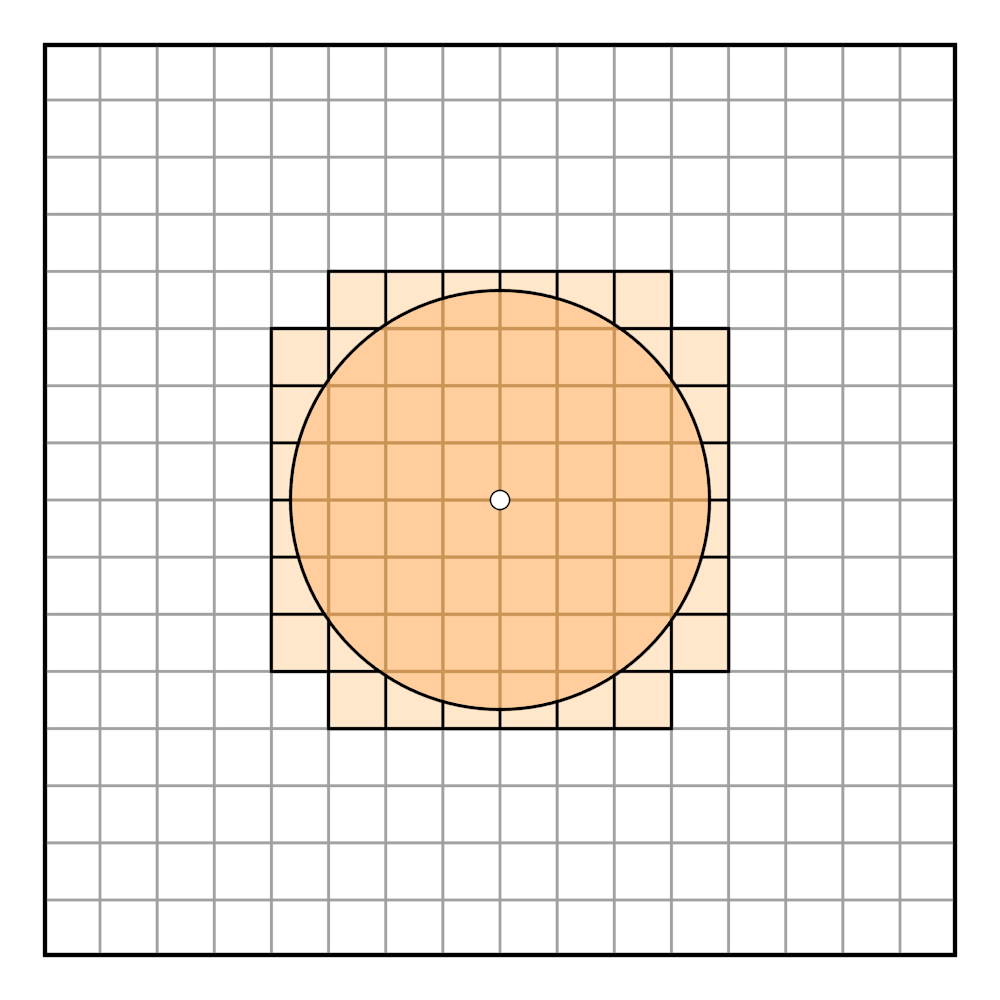
\includegraphics[width=\textwidth]{./img/raw/dl-transformations/1.png}
    \caption{Het licht.}
    \label{fig:dl-transformaties:base}
  \end{subfigure}%
  \begin{subfigure}[b]{0.3\textwidth}
    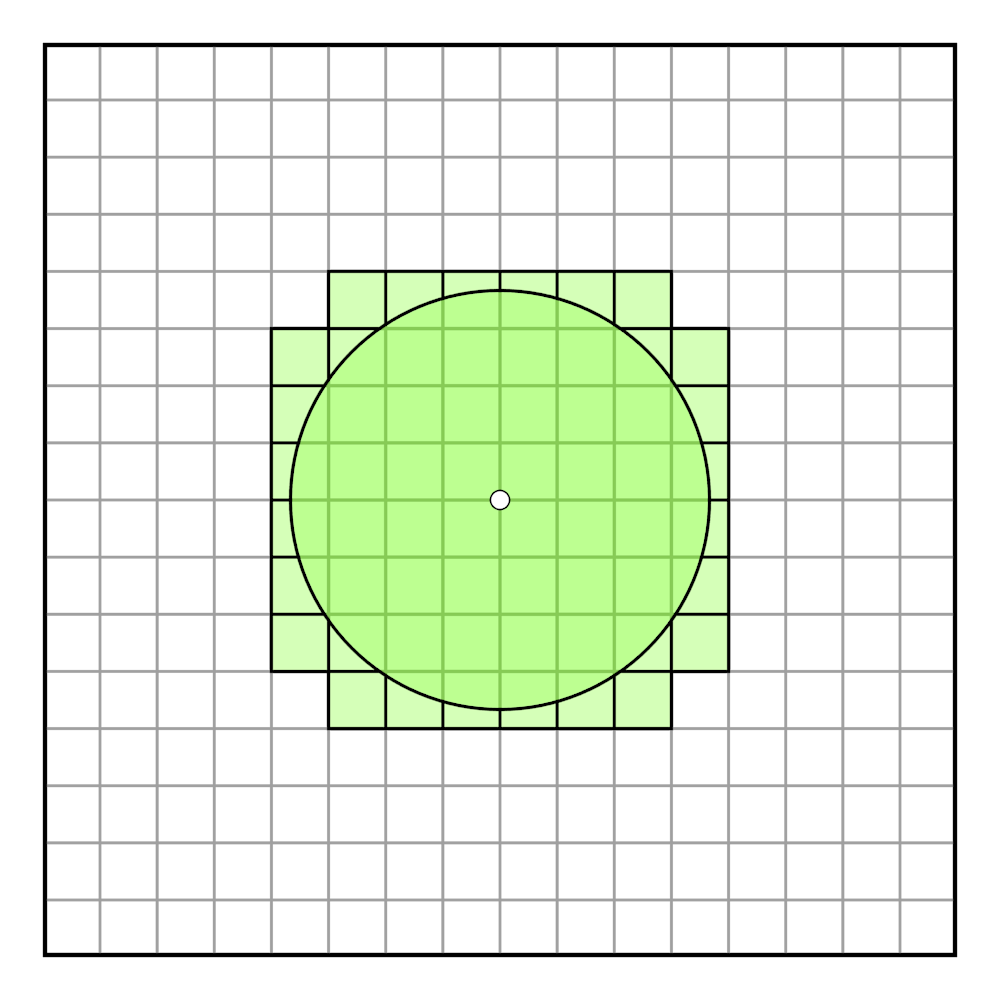
\includegraphics[width=\textwidth]{./img/raw/dl-transformations/add.png}
    \caption{Toevoegen.}
    \label{fig:dl-transformaties:add}
  \end{subfigure}%
  \begin{subfigure}[b]{0.3\textwidth}
    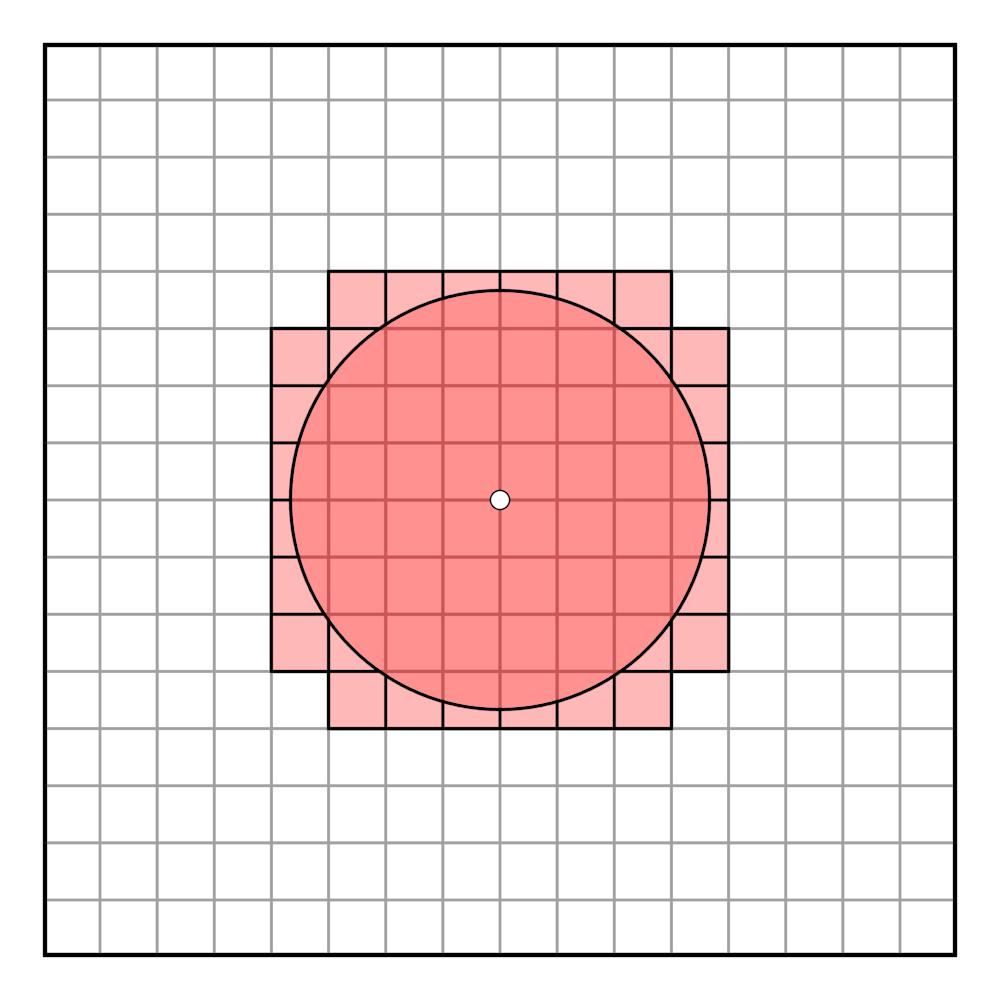
\includegraphics[width=\textwidth]{./img/raw/dl-transformations/remove.png}
    \caption{Verwijderen.}
    \label{fig:dl-transformaties:remove}
  \end{subfigure}\\
  \begin{subfigure}[b]{0.3\textwidth} %
    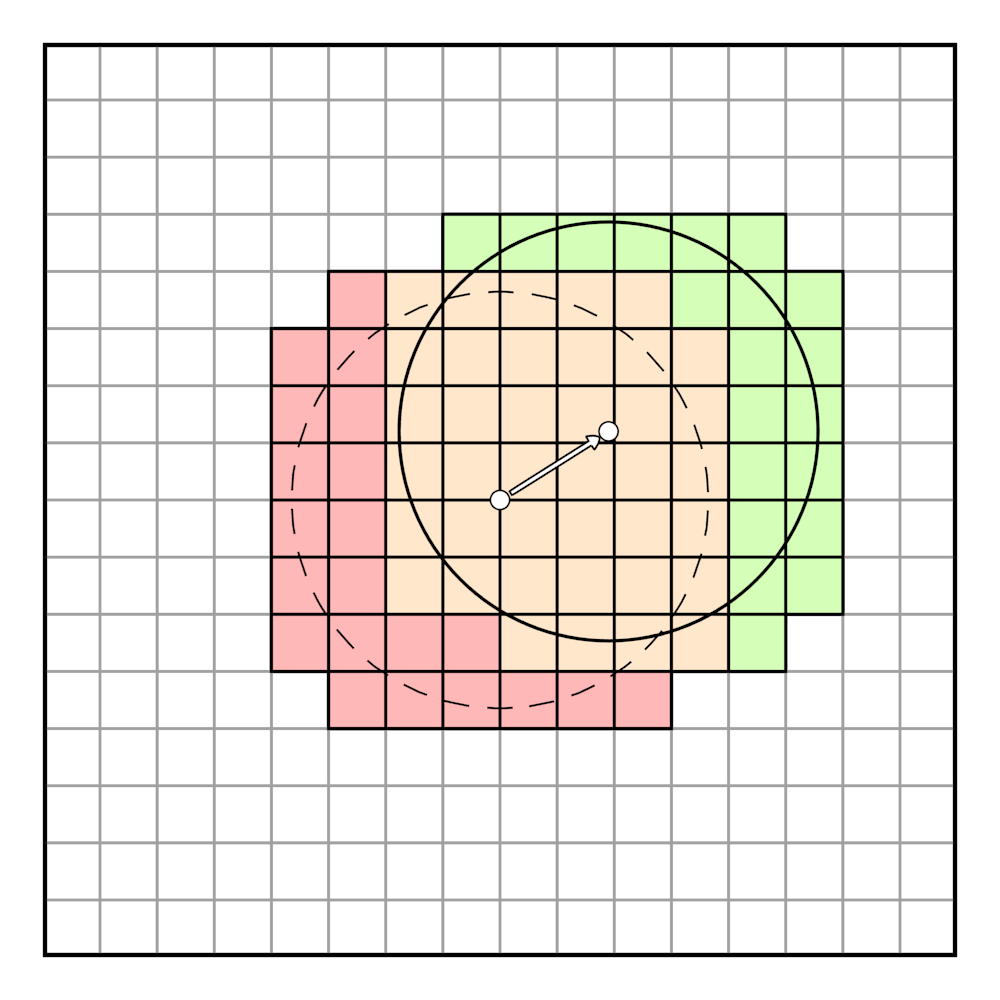
\includegraphics[width=\textwidth]{./img/raw/dl-transformations/translation.png}
    \caption{Transleren.}
    \label{fig:dl-transformaties:translate}
  \end{subfigure}%
  \begin{subfigure}[b]{0.3\textwidth}
    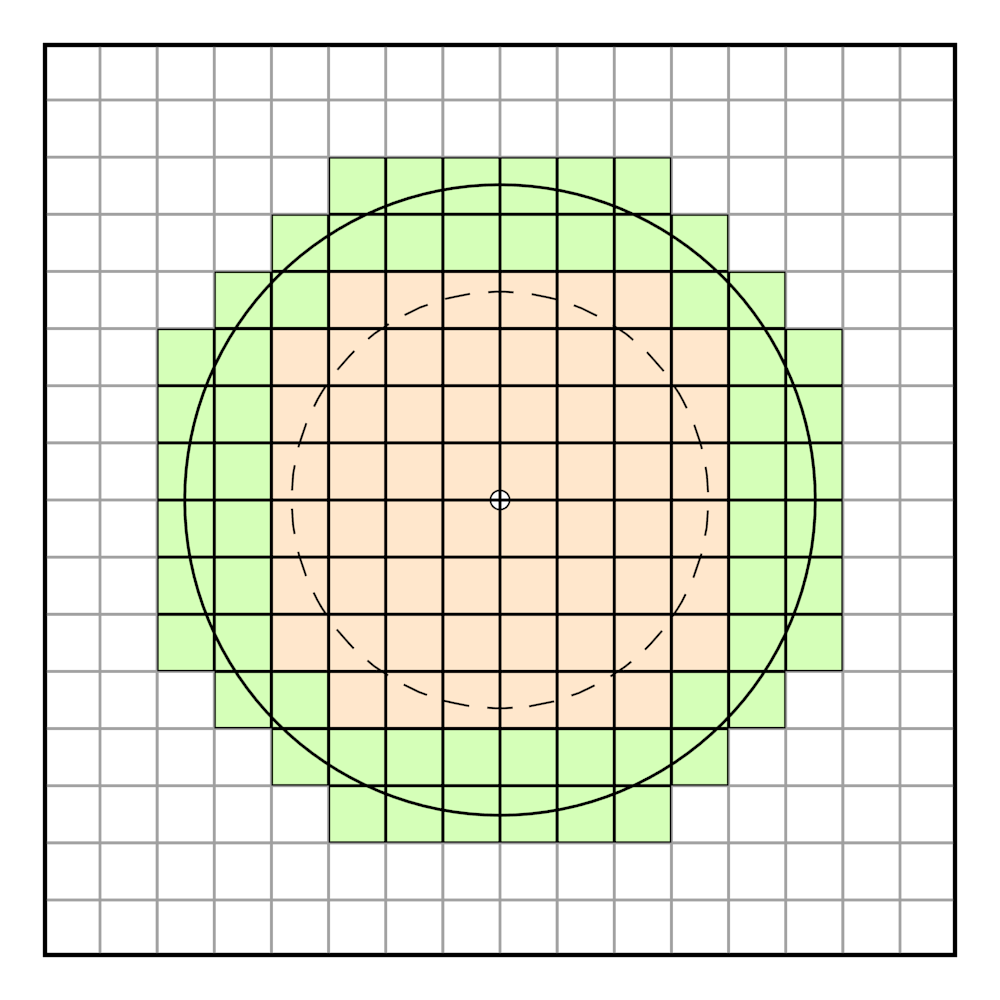
\includegraphics[width=\textwidth]{./img/raw/dl-transformations/scale_up.png}
    \caption{Vergroten van de radius.}
    \label{fig:dl-transformaties:scale-up}
  \end{subfigure}%
  \begin{subfigure}[b]{0.3\textwidth}
    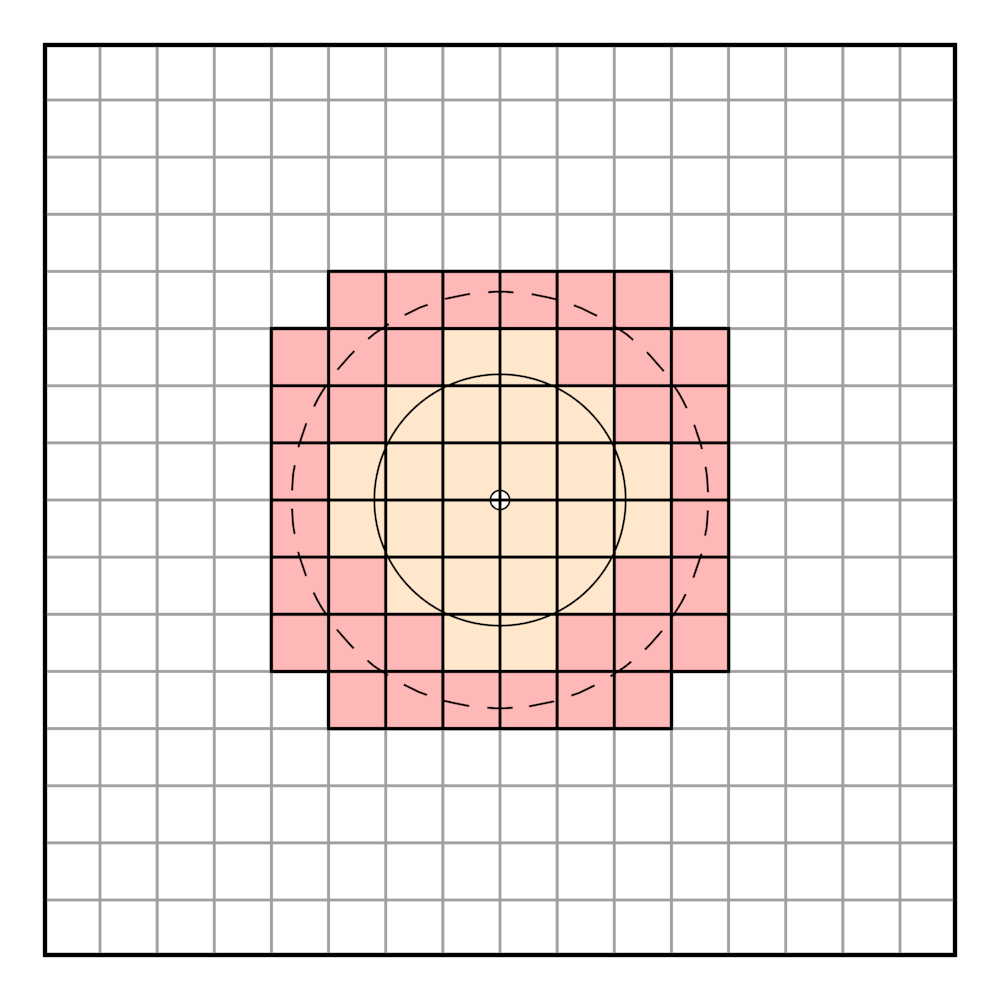
\includegraphics[width=\textwidth]{./img/raw/dl-transformations/scale_down.png}
    \caption{Verkleinen van de radius.}
    \label{fig:dl-transformaties:scale-down}
  \end{subfigure}
  \caption{2D weergave van de mogelijke transformaties van puntlichten en hun invloed op de octree structuur.}
  \label{fig:dl-transformaties}
\end{figure}

